\begin{figure}[!h]
\centering
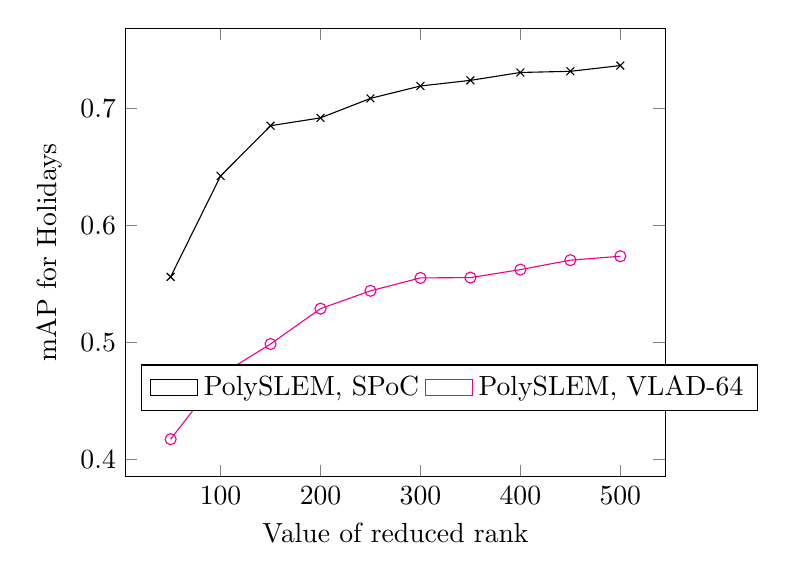
\begin{tikzpicture}
	\begin{axis}[
		xlabel=Value of reduced rank,
		ylabel=mAP for Holidays,
		legend style={
			area legend,
			at={(0.6,0.25)},
			anchor=north,
			legend columns=-1}]
%%Poly SLEM
    \addplot[mark=x, black] coordinates{
        (  50, 0.5560)
        ( 100, 0.6421)
        ( 150, 0.6850)
        ( 200, 0.6917)
         (250, 0.7083)
         (300, 0.7189)
         (350, 0.7237)
      (   400, 0.73043)
      (   450, 0.73143)
      (   500, 0.73631)
    };
    \addlegendentry{PolySLEM, SPoC}
    \addplot[mark=o, magenta] coordinates{
        (  50, 0.4175)
        ( 100, 0.4723)
        ( 150, 0.4987)
        ( 200, 0.5289)
       (  250, 0.5441)
       (  300, 0.55512)
       (  350, 0.55540)
      (   400, 0.56221)
      (   450, 0.57027)
      (   500, 0.57361)
    };
    \addlegendentry{PolySLEM, VLAD-64}
	\end{axis}
\end{tikzpicture}
\caption{mAP for Holidays using SPoC and VLAD-64 features. We perform a low-rank decomposition of a $50000\times 50000$ kernel matrix.}
\end{figure}

